\section{addnewrecord Class Reference}
\label{classaddnewrecord}\index{addnewrecord@{addnewrecord}}
{\tt \#include $<$addnewrecord.h$>$}

Collaboration diagram for addnewrecord:\begin{figure}[H]
\begin{center}
\leavevmode
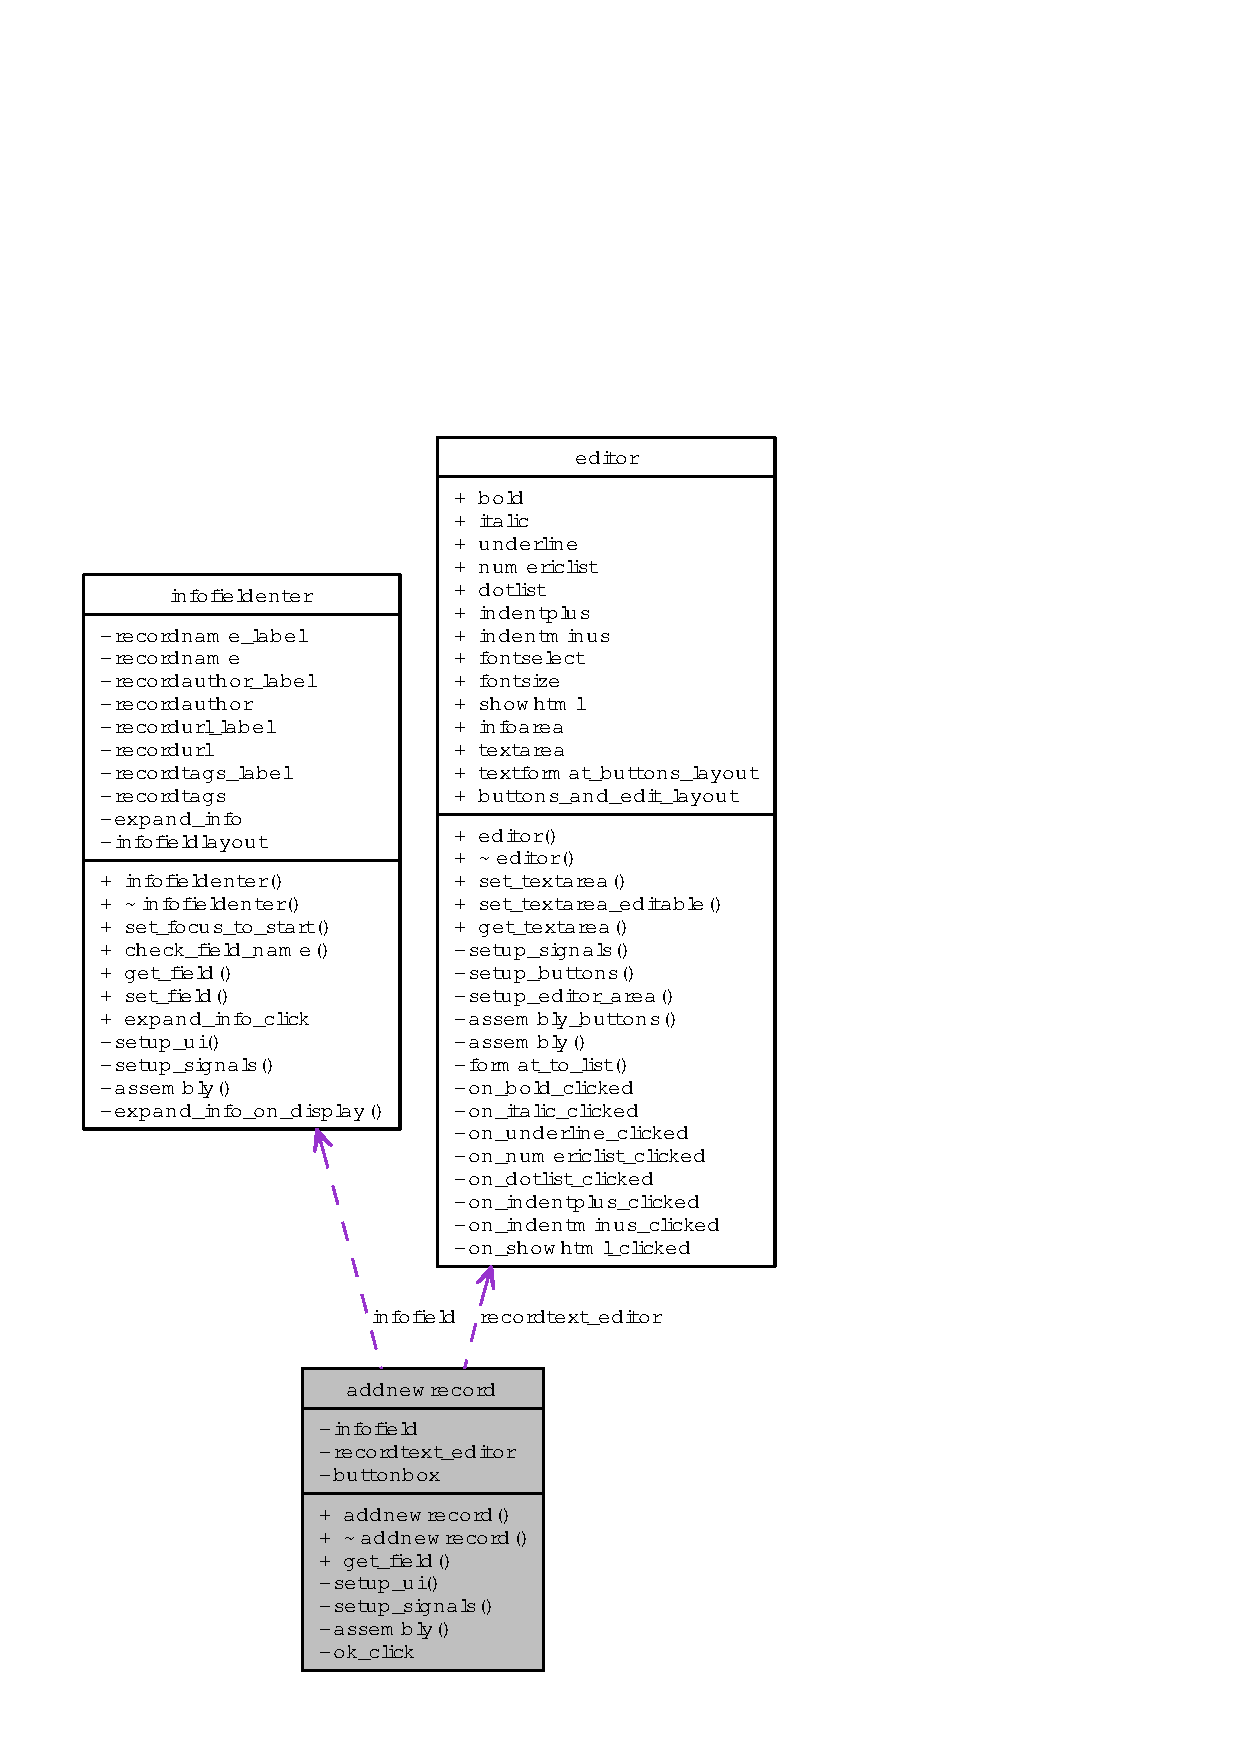
\includegraphics[width=191pt]{classaddnewrecord__coll__graph}
\end{center}
\end{figure}
\subsection*{Public Member Functions}
\begin{CompactItemize}
\item 
{\bf addnewrecord} (QWidget $\ast$parent=0, Qt::WFlags f=0)
\item 
{\bf $\sim$addnewrecord} ()
\item 
QString {\bf get\_\-field} (QString name)
\end{CompactItemize}
\subsection*{Private Slots}
\begin{CompactItemize}
\item 
void {\bf ok\_\-click} (void)
\end{CompactItemize}
\subsection*{Private Member Functions}
\begin{CompactItemize}
\item 
void {\bf setup\_\-ui} (void)
\item 
void {\bf setup\_\-signals} (void)
\item 
void {\bf assembly} (void)
\end{CompactItemize}
\subsection*{Private Attributes}
\begin{CompactItemize}
\item 
{\bf infofieldenter} $\ast$ {\bf infofield}
\item 
{\bf editor} $\ast$ {\bf recordtext\_\-editor}
\item 
QDialog\-Button\-Box $\ast$ {\bf buttonbox}
\end{CompactItemize}


\subsection{Detailed Description}




Definition at line 16 of file addnewrecord.h.

\subsection{Constructor \& Destructor Documentation}
\index{addnewrecord@{addnewrecord}!addnewrecord@{addnewrecord}}
\index{addnewrecord@{addnewrecord}!addnewrecord@{addnewrecord}}
\subsubsection{\setlength{\rightskip}{0pt plus 5cm}addnewrecord::addnewrecord (QWidget $\ast$ {\em parent} = {\tt 0}, Qt::WFlags {\em f} = {\tt 0})}\label{classaddnewrecord_729e13e04194b13db2db349baa0c83b4}




Definition at line 13 of file addnewrecord.cpp.

References assembly(), setup\_\-signals(), and setup\_\-ui().

Here is the call graph for this function:\begin{figure}[H]
\begin{center}
\leavevmode
\includegraphics[width=315pt]{classaddnewrecord_729e13e04194b13db2db349baa0c83b4_cgraph}
\end{center}
\end{figure}
\index{addnewrecord@{addnewrecord}!~addnewrecord@{$\sim$addnewrecord}}
\index{~addnewrecord@{$\sim$addnewrecord}!addnewrecord@{addnewrecord}}
\subsubsection{\setlength{\rightskip}{0pt plus 5cm}addnewrecord::$\sim$addnewrecord ()}\label{classaddnewrecord_bf0eb3a43fdb46e529beb06212aaab06}




Definition at line 20 of file addnewrecord.cpp.

\subsection{Member Function Documentation}
\index{addnewrecord@{addnewrecord}!get_field@{get\_\-field}}
\index{get_field@{get\_\-field}!addnewrecord@{addnewrecord}}
\subsubsection{\setlength{\rightskip}{0pt plus 5cm}QString addnewrecord::get\_\-field (QString {\em name})}\label{classaddnewrecord_b17a7bac9ffb0b9474e0c5a50eecd958}




Definition at line 102 of file addnewrecord.cpp.

References infofieldenter::get\_\-field(), editor::get\_\-textarea(), infofield, and recordtext\_\-editor.

Referenced by recordtablescreen::add\_\-new\_\-record(), and ok\_\-click().

Here is the call graph for this function:\begin{figure}[H]
\begin{center}
\leavevmode
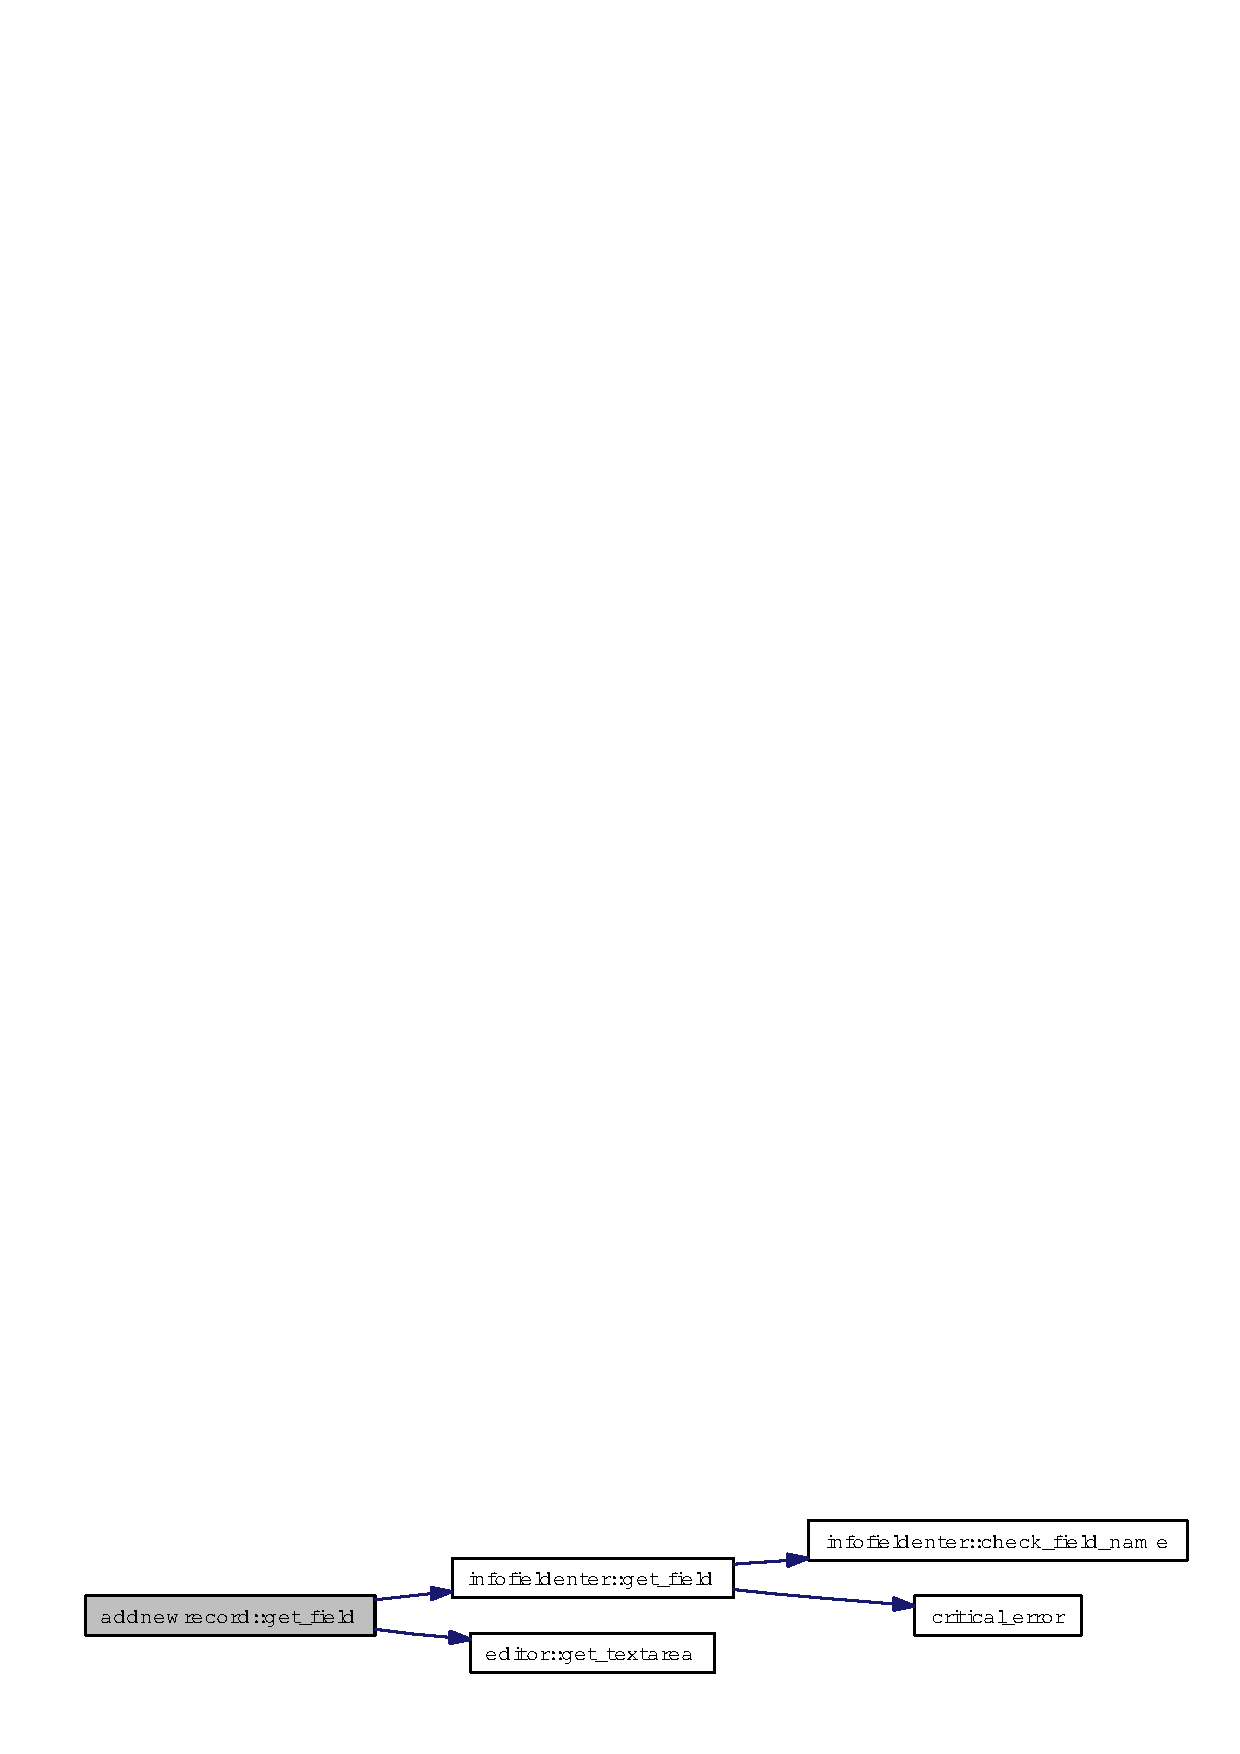
\includegraphics[width=287pt]{classaddnewrecord_b17a7bac9ffb0b9474e0c5a50eecd958_cgraph}
\end{center}
\end{figure}


Here is the caller graph for this function:\begin{figure}[H]
\begin{center}
\leavevmode
\includegraphics[width=209pt]{classaddnewrecord_b17a7bac9ffb0b9474e0c5a50eecd958_icgraph}
\end{center}
\end{figure}
\index{addnewrecord@{addnewrecord}!ok_click@{ok\_\-click}}
\index{ok_click@{ok\_\-click}!addnewrecord@{addnewrecord}}
\subsubsection{\setlength{\rightskip}{0pt plus 5cm}void addnewrecord::ok\_\-click (void)\hspace{0.3cm}{\tt  [private, slot]}}\label{classaddnewrecord_67eaa32fb215ac1ee6fa45f118bd26d9}




Definition at line 71 of file addnewrecord.cpp.

References get\_\-field(), infofieldenter::get\_\-field(), and infofield.

Referenced by setup\_\-signals().\index{addnewrecord@{addnewrecord}!setup_ui@{setup\_\-ui}}
\index{setup_ui@{setup\_\-ui}!addnewrecord@{addnewrecord}}
\subsubsection{\setlength{\rightskip}{0pt plus 5cm}void addnewrecord::setup\_\-ui (void)\hspace{0.3cm}{\tt  [private]}}\label{classaddnewrecord_80133fefeb4b5d183232f13b6d96ca60}




Definition at line 26 of file addnewrecord.cpp.

References buttonbox, ENABLE\_\-ASSEMBLY, infofield, and recordtext\_\-editor.

Referenced by addnewrecord().

Here is the caller graph for this function:\begin{figure}[H]
\begin{center}
\leavevmode
\includegraphics[width=193pt]{classaddnewrecord_80133fefeb4b5d183232f13b6d96ca60_icgraph}
\end{center}
\end{figure}
\index{addnewrecord@{addnewrecord}!setup_signals@{setup\_\-signals}}
\index{setup_signals@{setup\_\-signals}!addnewrecord@{addnewrecord}}
\subsubsection{\setlength{\rightskip}{0pt plus 5cm}void addnewrecord::setup\_\-signals (void)\hspace{0.3cm}{\tt  [private]}}\label{classaddnewrecord_16b5cb93b2861de3fb4da880a09a683f}




Definition at line 42 of file addnewrecord.cpp.

References buttonbox, and ok\_\-click().

Referenced by addnewrecord().

Here is the caller graph for this function:\begin{figure}[H]
\begin{center}
\leavevmode
\includegraphics[width=206pt]{classaddnewrecord_16b5cb93b2861de3fb4da880a09a683f_icgraph}
\end{center}
\end{figure}
\index{addnewrecord@{addnewrecord}!assembly@{assembly}}
\index{assembly@{assembly}!addnewrecord@{addnewrecord}}
\subsubsection{\setlength{\rightskip}{0pt plus 5cm}void addnewrecord::assembly (void)\hspace{0.3cm}{\tt  [private]}}\label{classaddnewrecord_303c727d43461d35848dfa41477899b3}




Definition at line 48 of file addnewrecord.cpp.

References buttonbox, infofield, recordtext\_\-editor, and infofieldenter::set\_\-focus\_\-to\_\-start().

Referenced by addnewrecord().

Here is the call graph for this function:\begin{figure}[H]
\begin{center}
\leavevmode
\includegraphics[width=203pt]{classaddnewrecord_303c727d43461d35848dfa41477899b3_cgraph}
\end{center}
\end{figure}


Here is the caller graph for this function:\begin{figure}[H]
\begin{center}
\leavevmode
\includegraphics[width=196pt]{classaddnewrecord_303c727d43461d35848dfa41477899b3_icgraph}
\end{center}
\end{figure}


\subsection{Member Data Documentation}
\index{addnewrecord@{addnewrecord}!infofield@{infofield}}
\index{infofield@{infofield}!addnewrecord@{addnewrecord}}
\subsubsection{\setlength{\rightskip}{0pt plus 5cm}{\bf infofieldenter}$\ast$ {\bf addnewrecord::infofield}\hspace{0.3cm}{\tt  [private]}}\label{classaddnewrecord_5f573afbfe718aefdd10d4750cca6337}




Definition at line 33 of file addnewrecord.h.

Referenced by assembly(), get\_\-field(), ok\_\-click(), and setup\_\-ui().\index{addnewrecord@{addnewrecord}!recordtext_editor@{recordtext\_\-editor}}
\index{recordtext_editor@{recordtext\_\-editor}!addnewrecord@{addnewrecord}}
\subsubsection{\setlength{\rightskip}{0pt plus 5cm}{\bf editor}$\ast$ {\bf addnewrecord::recordtext\_\-editor}\hspace{0.3cm}{\tt  [private]}}\label{classaddnewrecord_fe979c440192b2306b4c895b9b4f6107}




Definition at line 36 of file addnewrecord.h.

Referenced by assembly(), get\_\-field(), and setup\_\-ui().\index{addnewrecord@{addnewrecord}!buttonbox@{buttonbox}}
\index{buttonbox@{buttonbox}!addnewrecord@{addnewrecord}}
\subsubsection{\setlength{\rightskip}{0pt plus 5cm}QDialog\-Button\-Box$\ast$ {\bf addnewrecord::buttonbox}\hspace{0.3cm}{\tt  [private]}}\label{classaddnewrecord_7f1498c7dede5dd0458b9efc867ddaa7}




Definition at line 38 of file addnewrecord.h.

Referenced by assembly(), setup\_\-signals(), and setup\_\-ui().

The documentation for this class was generated from the following files:\begin{CompactItemize}
\item 
{\bf addnewrecord.h}\item 
{\bf addnewrecord.cpp}\end{CompactItemize}
